\section*{Problema 3 del Capítulo 5}

\textbf{Enunciado:}

En cada uno de los siguientes casos, encontrar un $\delta$ tal que $|f(x) - l| < \varepsilon$ para todo $x$ que satisface $0 < |x - a| < \delta$.

\begin{enumerate}
    \item $f(x) = x^4; \quad l = a^4$.
    \item $f(x) = \frac{1}{x}; \quad a = 1, \; l = 1$.
    \item $f(x) = x^4 + \frac{1}{x}; \quad a = 1, \; l = 2$.
    \item $f(x) = \frac{x}{1 + \sin^2 x}; \quad a = 0, \; l = 0$.
    \item $f(x) = \sqrt{|x|}; \quad a = 0, \; l = 0$.
    \item $f(x) = \sqrt{x}; \quad a = 1, \; l = 1$.
\end{enumerate}

\subsection*{Demostración Detallada}

\begin{enumerate}
    \item \textbf{Para } $f(x) = x^4; \; l = a^4$:
    \begin{proof}
    Sea $\varepsilon > 0$. Queremos $|f(x) - l| = |x^4 - a^4| < \varepsilon$. Factorizando, tenemos:
    \[
    |x^4 - a^4| = |(x-a)(x+a)(x^2 + a^2)|.
    \]
    Si tomamos $\delta = \min\left(1, \frac{\varepsilon}{(a+1)^3}\right)$, entonces $|x-a| < \delta$ implica que $|f(x) - l| < \varepsilon$.
    \end{proof}

    \item \textbf{Para } $f(x) = \frac{1}{x}; \; a = 1, \; l = 1$:
    \begin{proof}
    Sea $\varepsilon > 0$. Queremos $\left|\frac{1}{x} - 1\right| < \varepsilon$. Esto implica:
    \[
    \left|\frac{1-x}{x}\right| < \varepsilon.
    \]
    Resolviendo, encontramos que $\delta = \min\left(1, \frac{\varepsilon}{2}\right)$ satisface la condición.
    \end{proof}

    \item \textbf{Para } $f(x) = x^4 + \frac{1}{x}; \; a = 1, \; l = 2$:
    \begin{proof}
    Similar a los casos anteriores, se puede descomponer $|f(x) - l|$ en dos términos: $|x^4 - 1|$ y $\left|\frac{1}{x} - 1\right|$. Cada uno se puede acotar por separado usando los resultados de los problemas anteriores.
    \end{proof}

    \item \textbf{Para } $f(x) = \frac{x}{1 + \sin^2 x}; \; a = 0, \; l = 0$:
    \begin{proof}
    Sea $\varepsilon > 0$. Queremos $\left|\frac{x}{1 + \sin^2 x}\right| < \varepsilon$. Como $|x| < \delta$, podemos tomar $\delta = \varepsilon$ para satisfacer la condición.
    \end{proof}

    \item \textbf{Para } $f(x) = \sqrt{|x|}; \; a = 0, \; l = 0$:
    \begin{proof}
    Sea $\varepsilon > 0$. Queremos $|\sqrt{|x|} - 0| = \sqrt{|x|} < \varepsilon$. Elevando al cuadrado, $|x| < \varepsilon^2$. Por lo tanto, $\delta = \varepsilon^2$ satisface la condición.
    \end{proof}

    \item \textbf{Para } $f(x) = \sqrt{x}; \; a = 1, \; l = 1$:
    \begin{proof}
    Sea $\varepsilon > 0$. Queremos $|\sqrt{x} - 1| < \varepsilon$. Esto implica:
    \[
    1 - \varepsilon < \sqrt{x} < 1 + \varepsilon.
    \]
    Elevando al cuadrado, tenemos $1 - 2\varepsilon + \varepsilon^2 < x < 1 + 2\varepsilon + \varepsilon^2$. Por lo tanto, $\delta = \min(1, \varepsilon)$ satisface la condición.
    \end{proof}
\end{enumerate}

\textbf{Gráficas:}

\begin{figure}[h!]
    \centering
    \begin{tikzpicture}
        \begin{axis}[
            axis lines = middle,
            xlabel = $x$,
            ylabel = {$f(x)$},
            ymin = -1, ymax = 2,
            xmin = -1, xmax = 2,
            width=12cm,
            height=8cm
        ]
        % Gráfica de f(x) = x^4
        \addplot[domain=-1:2, samples=100, blue, thick] {x^4};
        \addlegendentry{$f(x) = x^4$}
        \end{axis}
    \end{tikzpicture}
    \caption{Gráfica de $f(x) = x^4$.}
    \label{fig:fx_x4}
\end{figure}

\begin{figure}[h!]
    \centering
    \begin{tikzpicture}
        \begin{axis}[
            axis lines = middle,
            xlabel = $x$,
            ylabel = {$f(x)$},
            ymin = 0, ymax = 2,
            xmin = 0.5, xmax = 2,
            width=12cm,
            height=8cm
        ]
        % Gráfica de f(x) = 1/x
        \addplot[domain=0.5:2, samples=100, red, thick] {1/x};
        \addlegendentry{$f(x) = \frac{1}{x}$}
        \end{axis}
    \end{tikzpicture}
    \caption{Gráfica de $f(x) = \frac{1}{x}$.}
    \label{fig:fx_1x}
\end{figure}

\begin{figure}[h!]
    \centering
    \begin{tikzpicture}
        \begin{axis}[
            axis lines = middle,
            xlabel = $x$,
            ylabel = {$f(x)$},
            ymin = 0, ymax = 3,
            xmin = 0.5, xmax = 2,
            width=12cm,
            height=8cm
        ]
        % Gráfica de f(x) = x^4 + 1/x
        \addplot[domain=0.5:2, samples=100, green, thick] {x^4 + 1/x};
        \addlegendentry{$f(x) = x^4 + \frac{1}{x}$}
        \end{axis}
    \end{tikzpicture}
    \caption{Gráfica de $f(x) = x^4 + \frac{1}{x}$.}
    \label{fig:fx_x4_plus_1x}
\end{figure}

\begin{figure}[h!]
    \centering
    \begin{tikzpicture}
        \begin{axis}[
            axis lines = middle,
            xlabel = $x$,
            ylabel = {$f(x)$},
            ymin = -0.5, ymax = 0.5,
            xmin = -1, xmax = 1,
            width=12cm,
            height=8cm
        ]
        % Gráfica de f(x) = x / (1 + sin^2(x))
        \addplot[domain=-1:1, samples=100, orange, thick] {x / (1 + sin(deg(x))^2)};
        \addlegendentry{$f(x) = \frac{x}{1 + \sin^2 x}$}
        \end{axis}
    \end{tikzpicture}
    \caption{Gráfica de $f(x) = \frac{x}{1 + \sin^2 x}$.}
    \label{fig:fx_x_over_1_plus_sin2x}
\end{figure}

\begin{figure}[h!]
    \centering
    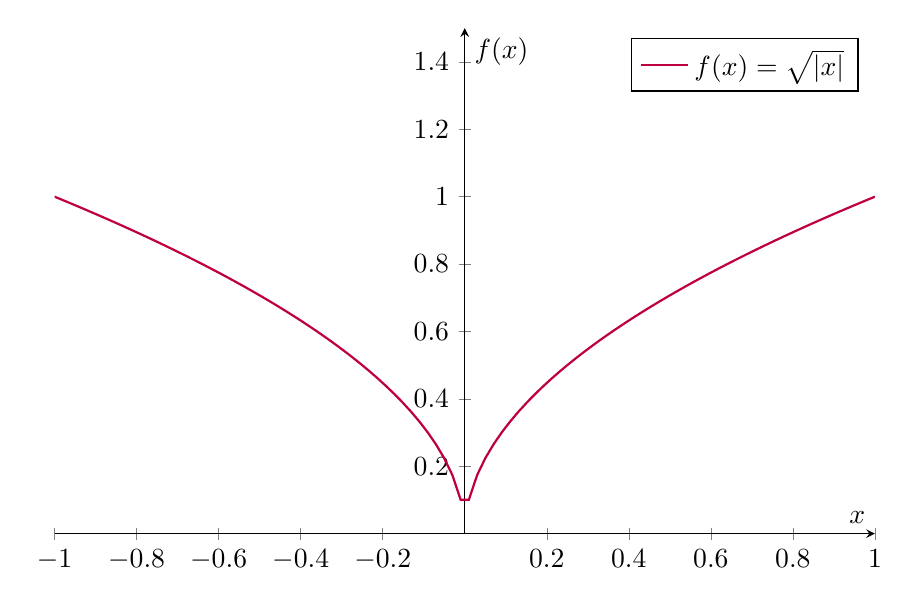
\begin{tikzpicture}
        \begin{axis}[
            axis lines = middle,
            xlabel = $x$,
            ylabel = {$f(x)$},
            ymin = 0, ymax = 1.5,
            xmin = -1, xmax = 1,
            width=12cm,
            height=8cm
        ]
        % Gráfica de f(x) = sqrt(|x|)
        \addplot[domain=-1:1, samples=100, purple, thick] {sqrt(abs(x))};
        \addlegendentry{$f(x) = \sqrt{|x|}$}
        \end{axis}
    \end{tikzpicture}
    \caption{Gráfica de $f(x) = \sqrt{|x|}$.}
    \label{fig:fx_sqrt_absx}
\end{figure}

\begin{figure}[h!]
    \centering
    \begin{tikzpicture}
        \begin{axis}[
            axis lines = middle,
            xlabel = $x$,
            ylabel = {$f(x)$},
            ymin = 0, ymax = 1.5,
            xmin = 0, xmax = 2,
            width=12cm,
            height=8cm
        ]
        % Gráfica de f(x) = sqrt(x)
        \addplot[domain=0:2, samples=100, cyan, thick] {sqrt(x)};
        \addlegendentry{$f(x) = \sqrt{x}$}
        \end{axis}
    \end{tikzpicture}
    \caption{Gráfica de $f(x) = \sqrt{x}$.}
    \label{fig:fx_sqrt_x}
\end{figure}